\chapter{Durchführung}
% =================================================================
\thispagestyle{fancy} \label{chap:durchfuehrung}
% =================================================================
\section{Versuchsaufbau}
In der Abbildung \ref{fig:versuchsaufbau} ist der komplette Versuchsaufbau zu sehen. Dabei wird das Fahrbahnpendel vom Gleiter (gelb markiert) repräsentiert und ist beidseitig mit jeweils einer Feder versehen, welche die Schwingungen kausieren. Das Fahrbahnpendel kann über eine Exzenterscheibe angeregt und Anhand dessen Lichtschranke II) am Zeitmessgerät über die Periodendauer die Erregerfrequenz ermittelt werden. Die durch induzierte Wirbelströme realisierte geschwindigkeitsproportionale Dämpfung kann am Fahrbahnpendel mittels kleinen Scheibenmagneten (Bremsmagneten) eingestellt werden. Diese können in beidseitig symmetrisch angeordnete Bohrungen mit Spannfedern fixiert werden. Das Fahrbahnpendel befindet sich auf einer Schiene mit kleinen Löchern durch welche Luft strömt. Dadurch wird unter dem Fahrbahnpendel ein Luftkissen erzeugt, auf dem es hin- und hergleiten kann. Auf dem Fahrbahnpendel befindet sich ein Unterbrecher I), welcher die Lichtschranke I) an der Stelle durchläuft, wo das Fahrbahnpendel sich in Ruhlage befindet. Die Lichtschrankenlogik muss dafür so eingestellt werden, dass gleich eine ganze Periodendauer gemessen wird. Kurz zusammengefasst misst die Lichtschranke I) die Eigenfrequenz, und die Lichtschranke II) die Erregerfrequenz. Über ein Laser Distanzmessgerät wird die Fahrbahnpendelbewegung mit einer 50Hz Sampling-Rate aufgenommen. Der Frequenzgenerator ist der Frequenzgeber, um über den Schrittmotor die Excenterscheibe anzutreiben.
\\[0.5cm]
Im Unterkapitel \ref{subsec:messgeraete} in der Tabelle \ref{tab:messgeraete} sind alle beschriebenen Geräte aufgelistet.
\\[0.7cm]
\begin{figure}[h]
	\centering
	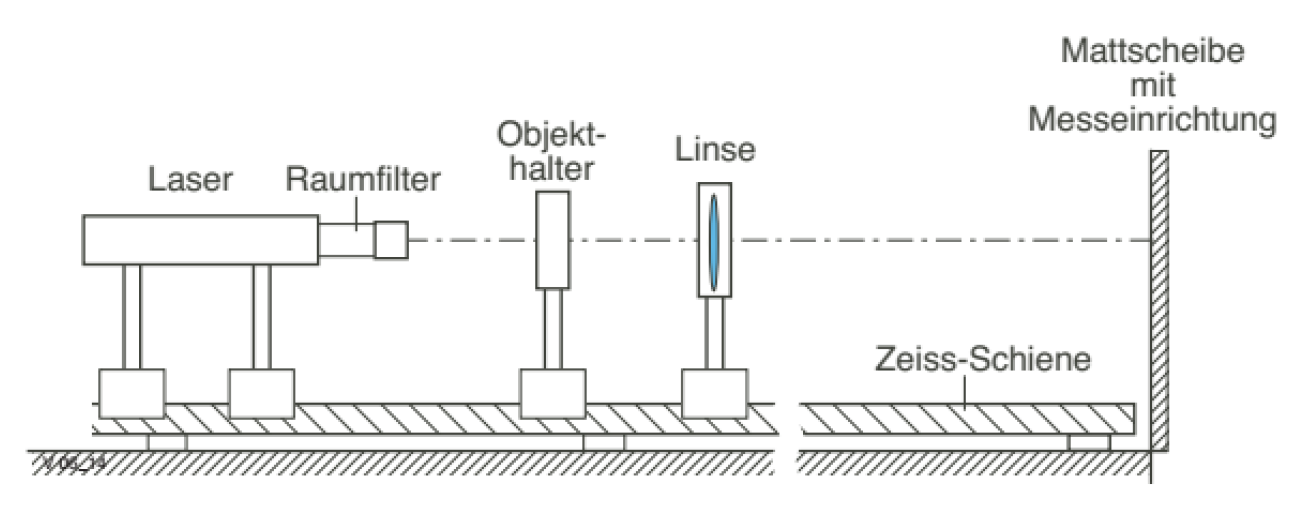
\includegraphics[width=17cm]{Bilder/versuchsaufbau.png} 
	\caption{Versuchsaufbau des Fahrbahnpendels mit Antriebs- und Messapparatur \cite{w6}}
	\label{fig:versuchsaufbau}
\end{figure}
\newpage
\subsection{Messgeräte}
\label{subsec:messgeraete}
\begin{table}[h]
\centering
	\begin{tabular}{lll} 
	\textbf{Gerätebezeichung} & \textbf{Typ} & \textbf{Nr.} \\ 
	\toprule 
	Laser Distanzmessgerät & LDM42E & P-07-024.2 \\ 
	\hline 
	Lichtschranken & - & - \\ 
	\hline 
	Schrittmotortreiber & SMT 057.074.039 & P-Z-056 \\ 
	\hline 
	Zeitmessgerät (2 mal) & Keithley 775 & P-P3-019 \\ 
	\hline 
	Frequenzgenrator & SRS DS345 & P-E13-056 \\ 
	\bottomrule
	\end{tabular}
\caption{Liste der verwendeten Geräte}
\label{tab:messgeraete}
\end{table}
\section{Vorgehen bei den Messungen}
In diesem Versuch werden Eigenfrequenz und Amplitudenverlauf einer freien gedämpften Schwingung und Amplituden- und Phasenresonanz einer erzwungenen Schwingung eruiert. Dafür wird unterschiedlich vorgegangen.
\subsection{Bestimmung der Eigenfrequenz einer freien gedämpften Schwingung}
Mittels der Lichtschranke I) (Abbildung \ref{fig:versuchsaufbau}) wird die Schwingungsdauer des Fahrbahnpendels (Periodendauer \textit{T}) gemessen. Für eine genaue Messung muss diese vom Unterbrecher I) ausgelöst werden, wenn sich das Fahrbahnpendel in Ruhelage befindet. Dabei muss darauf geachtet werden, dass das Gestänge der Exzenterscheibe in Nulllage ist\footnote{kann mittels eines Stiftes befestigt werden}. Danach die Schattengrenze des Unterbrechers I) direkt auf die Mitte des Fotodetektors richten.
\\[0.5cm]
Der Betriebsmodus der Lichtschrankenlogik kann bei genügend grosser Auslenkung auf \glqq Pendel\grqq\: eingestellt werden. Ansonsten im Betriebsmodus \glqq Normal\grqq.
\subsection{Messung des Amplitudenverlaufs einer freien gedämpften Schwingung}
Die Auslenkung der Schwingungamplitude wird mit dem Laser Distanzmessgerät mit einer Sampling-Rate von 50Hz (50 Abtastwerte pro Sekunde) detektiert. Diese Werte werden dann auf einem vom Dozenten zur verfügung gestellten Computer im zeitlichen Verlauf geplottet. Durch schlechte kalibrierung des Clocks des Laser Distanzmessgerätes müssen die Zeitwerte mit einem Kalibrierungsfaktor angepasst werden. Dafür wird dieser mit der dem Abtastwert zugeordneten Zeit multipliziert. 
\subsection{Amplituden- und Phasenresonanz einer erzwungenen Schwingung}
Hier müssen beide Lichtschranken auf das gleiche Zeitmessgerät angeschlossen werden (Lichtschranke II) auf Channel A und Lichtschranke I) auf Channel B). Ca. 1200kHz beim Frequenzgenerator einstellen, und den Channel A auf dem Zeitmessgerät die Periodendauer $T$ der Exzenterscheibe ablesen. Damit kann die Erregerfrequenz nach $f_{e} = \frac{1}{T}$ berechnet werden. Gleichzeitig mit dem Laser Distanzmessgerät den Amplitudenverlauf des Fahrbahnpendels messen. Nach einer kurzen Zeit \glqq stabilisiert\grqq\: sich das System und es kann am Computer die Amplitude abgelesen werden\footnote{wenn der Amplitudenverlauf gleichmässig verläuft, hat sich das System stabilisiert}. Zusätzlich auf dem Zeitmessgerät die Phasendifferenz der Messungen der beiden Lichtschranken anzeigen lassen (A $\rightarrow$ B) und notieren. Dies nun für mehrere unterschiedliche Frequenzen des Frequenzgenerators wiederholen, um somit eine Amplitudenresonanzkurve wie in der Abbildung \ref{fig:erzwungeneSchwingung} zu erhalten.